\documentclass[../../labo_tp5_main.tex]{subfiles}

\begin{document}

%capítulo
\section{Ejercicio 8}

\subsection{Sinc}

Se observ\'o el espectro de una se\~nal de forma $x(t) = \frac{\sin{(\pi f \cdot t)}}{\pi f \cdot t} = \mathrm{sinc}(f\cdot t)$, con amplitud 250m$\mathrm{V}_{\mathrm{pp}}$ en la entrada del analizador, y frecuencia 125kHz. Por lo tanto, se espera observar en el mismo un pulso, que es su transformada de Fourier.

\begin{figure}[H]
	\centering
	\fbox{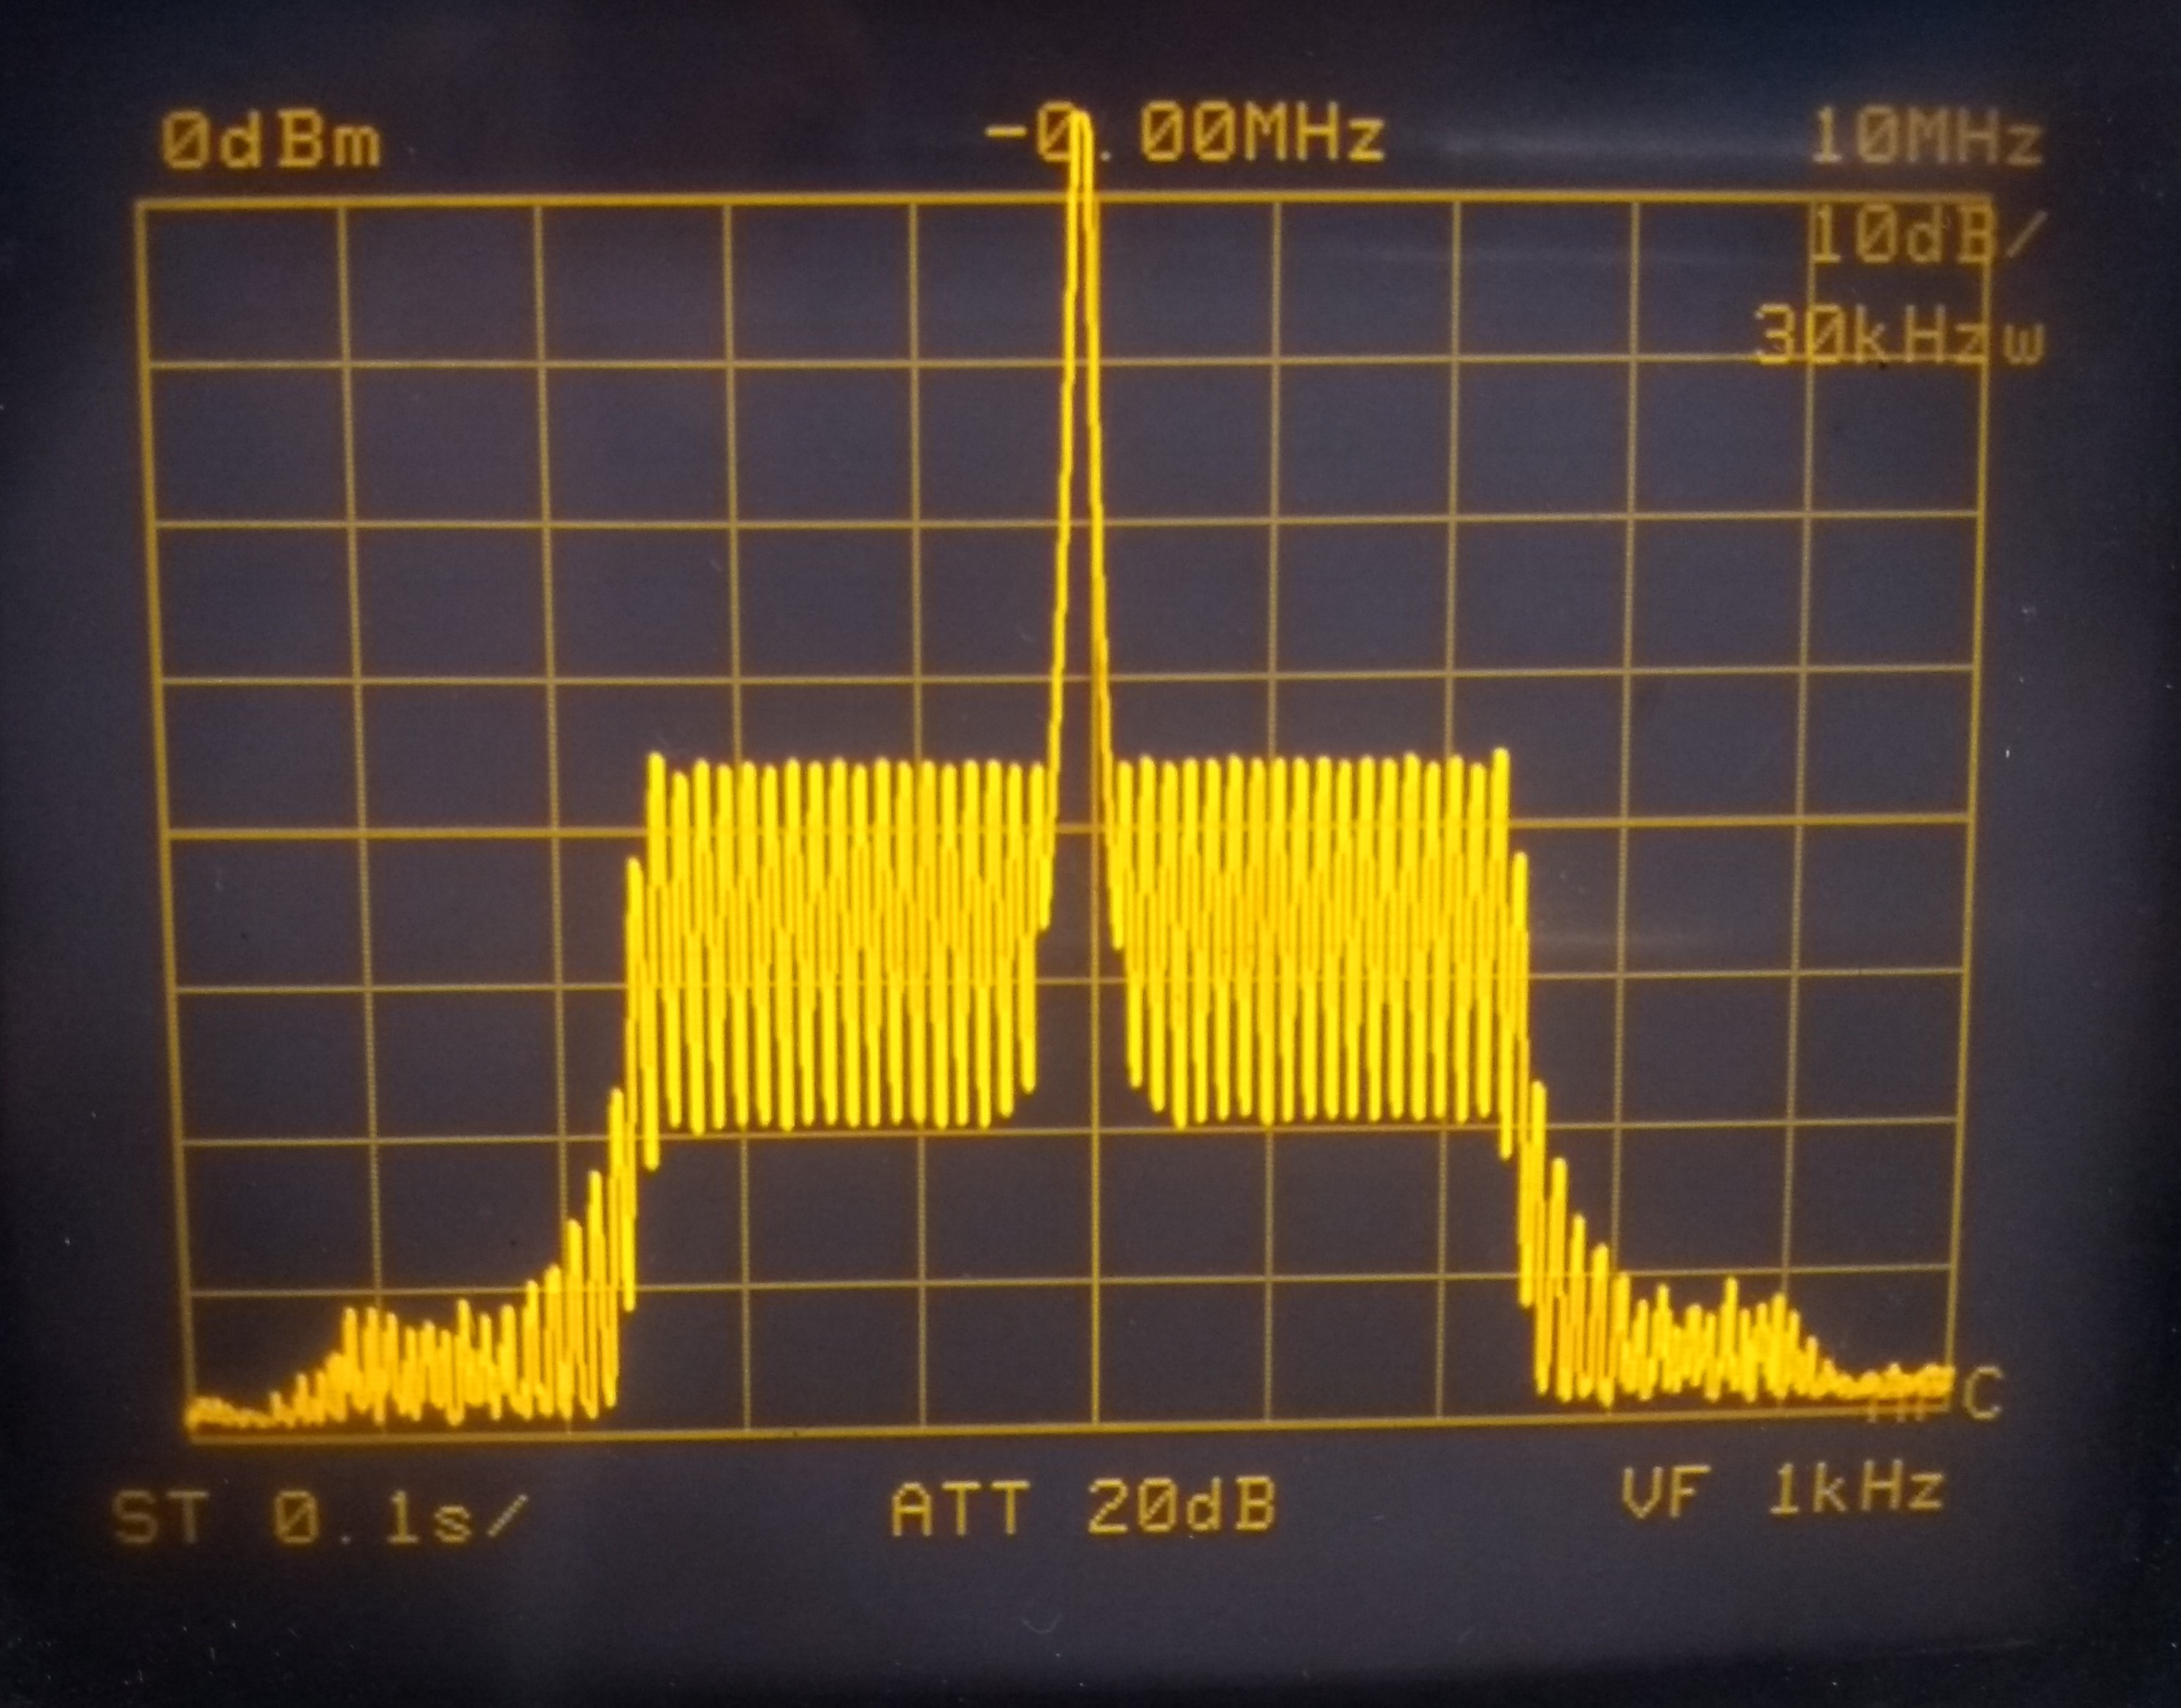
\includegraphics[scale=0.073]{imagenes/labo_tp5_ej8_sinc1.jpg}}
	\caption{Espectro del sinc}
\end{figure}

Este resultado es, entonces, consistente con lo que se esperaba observar.


\subsection{Tren de deltas}

Se procedi\'o a medir el espectro de un tren de deltas. En la pr\'actica, como es imposible obtener un delta, esta se\~nal consiste en un tren de pulsos del menor ancho que puede realizar el generador de funciones utilizado.

\begin{figure}[H]
	\centering
	\fbox{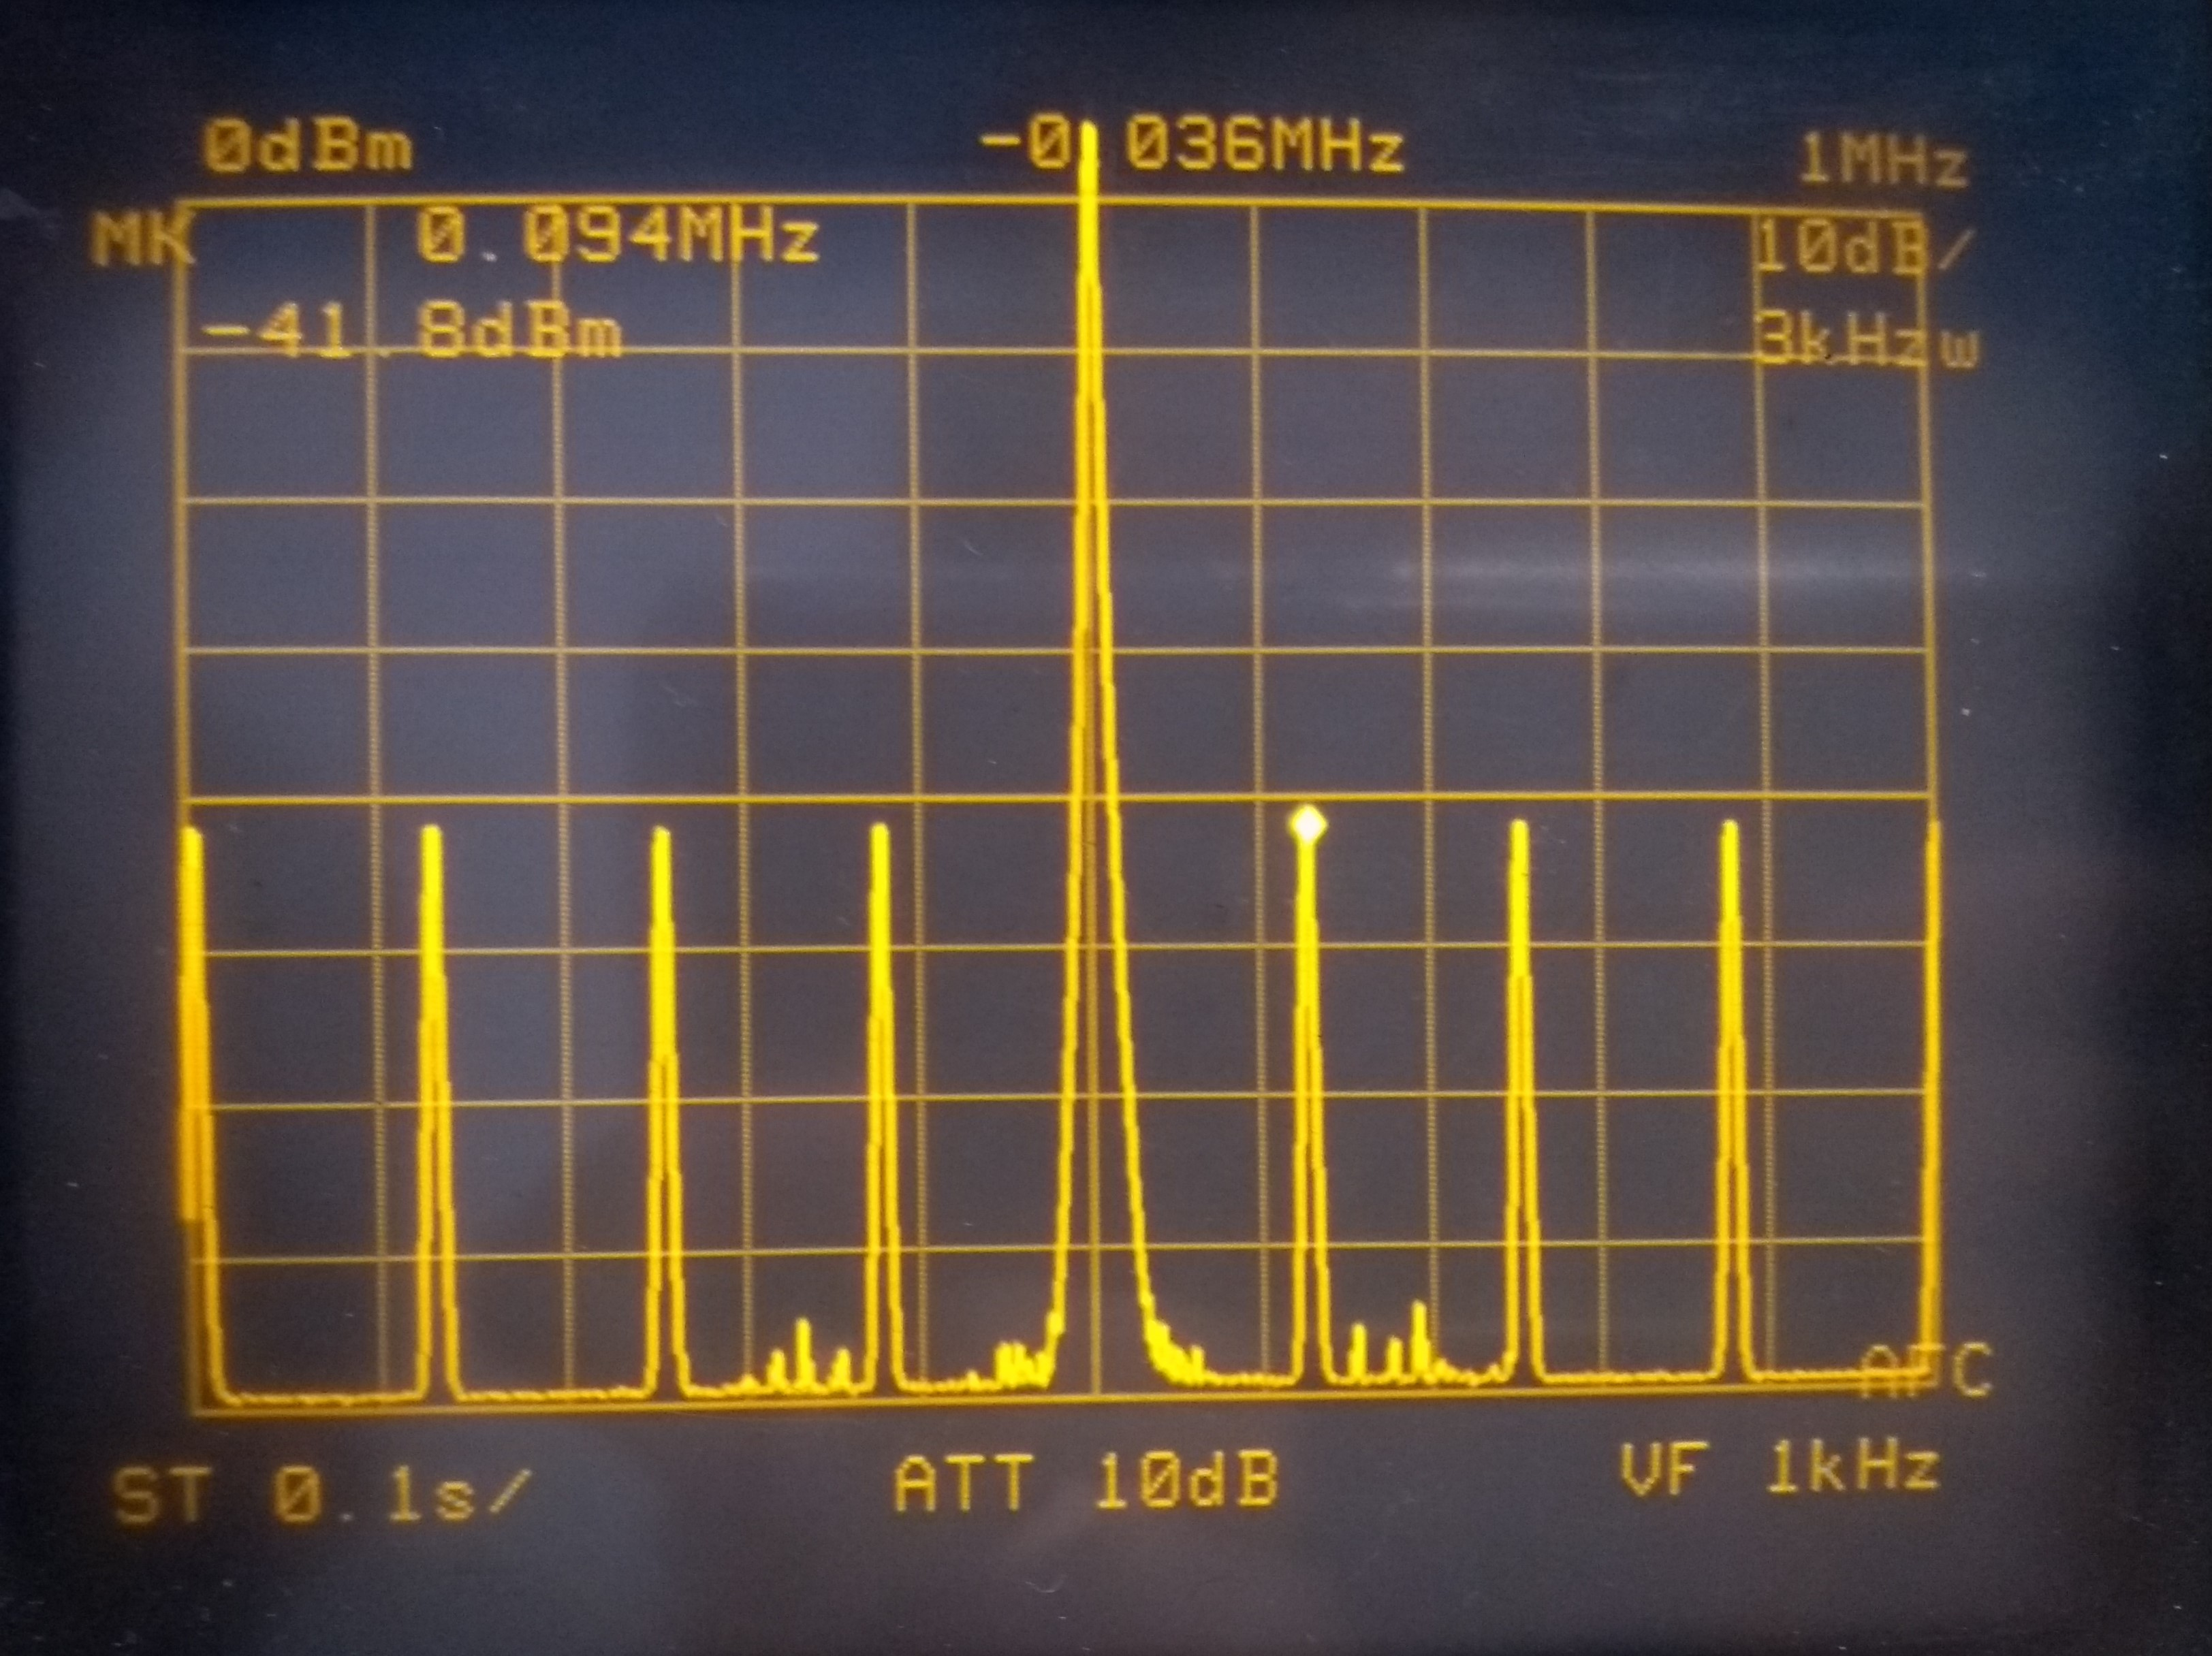
\includegraphics[scale=0.07]{imagenes/labo_tp5_ej8_deltas.jpg}}
	\caption{Espectro del tren de deltas}
\end{figure}

Al contrario de lo que ocurri\'o en el ejercicio 2, aqu\'i la diferencia en la potencia de los deltas obtenidos en el espectro no es apreciable, a pesar de que en ambos casos se trabaj\'o con se\~nales cuadradas. Esto indica que el duty cycle de la funci\'on generada en este caso es lo suficientemente peque\~no como para que el analizador lo perciba como un verdadero tren de deltas.



\end{document}
